\documentclass[11pt,a4paper]{article}
\usepackage[utf8]{inputenc}
\usepackage[T1]{fontenc}
\usepackage{graphicx,geometry,amsmath,longtable,hyperref}
\geometry{margin=2.0cm}
\hypersetup{colorlinks=true,urlcolor=blue,linkcolor=blue}
\setlength{\parindent}{0pt}
\setlength{\parskip}{0.5em}
\title{KFParticle $\Lambda$--$^{4}\mathrm{He}$\\Correlation Analysis: QA Summary}
\author{STAR analysis working report}
\date{2026-10-03 19:36 JST}
\begin{document}
\maketitle
\section{Sample and scope}
Au+Au fixed-target sample, beam-energy label 13.5 GeV; production 2020 P24iy. This beam label is \emph{not} a claim that $\sqrt{s_{NN}}$ equals this value.
\textbf{Partial merge:} 542/545 subjobs are included; 3 missing or excluded subjobs are not represented. No missing yield is filled in.
\par{\small\textbf{ROOT:} \path{auau13p5_anaFemtoLambda_4He_KFParticle_2020P24iy_partial_merge.root}\par
\textbf{SUMS ID:} \texttt{1213058CE62BCF113B2E3C75ACBD7053}\par}
This report reuses the structure of the earlier tools summaries, but reads only the KFParticle merged ROOT above. Legacy ROOTs, legacy PDFs and selection cuts are unchanged. The methods below are post-processing cross-checks, not new production selection or a final physics result.
\begin{center}\begin{tabular}{lr}\hline Measurement & Stored value\\\hline
Input-event counter & 36,004,989\\
Reconstructed-event counter & 34,883,141\\
Selected-$\Lambda$ counter & 3,044,144\\
Signal-window candidate counts & 2,463,680\\
Width-scaled sideband background & 50,103\\
Inclusive purity proxy $P$ & $0.979663\pm0.000055$\\\hline
\end{tabular}\end{center}
\begin{figure}[!ht]\centering
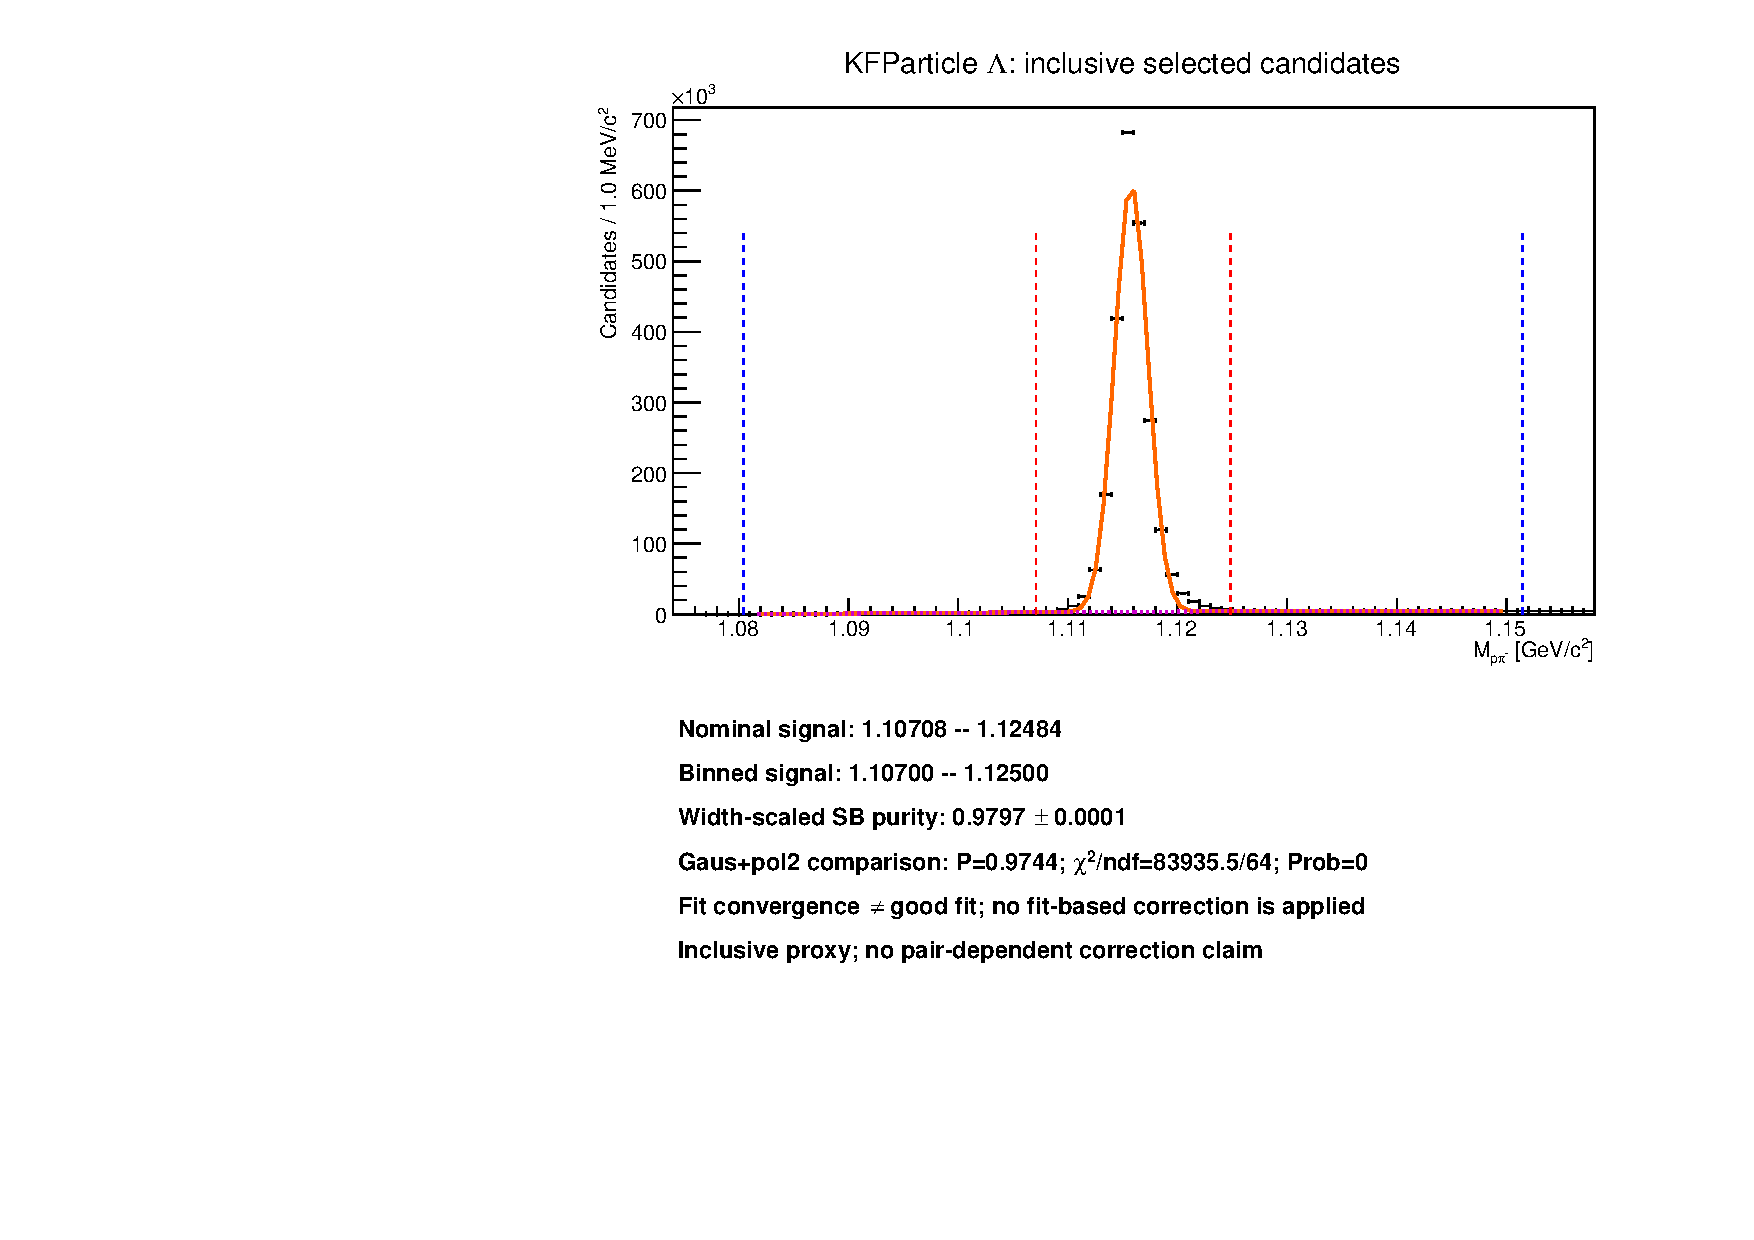
\includegraphics[width=0.58\textwidth,page=1]{Lambda_InvMass.pdf}
\caption{Inclusive $p\pi^-$ invariant mass. Vertical markers show the unchanged production signal and sideband gates; the fit is a diagnostic only.}
\end{figure}
\clearpage\section{Mass gates and purity convention}
The Maker gate parameters are $\mu=1.11596$ GeV/$c^2$, $\sigma=0.00296$ GeV/$c^2$, with signal $|M-\mu|<3\sigma$. The left/right sidebands extend from $3\sigma$ to $12\sigma$. These fixed gate parameters are not refitted to redefine the event selection.
\begin{center}\begin{tabular}{lcc}\hline Region & Nominal edges & Integrated bin edges\\\hline
Signal & 1.10708--1.12484 & 1.107--1.125\\
Left SB & 1.08044--1.10708 & 1.08--1.107\\
Right SB & 1.12484--1.15148 & 1.125--1.151\\
\hline\end{tabular}\end{center}
All mass edges are in GeV/$c^2$. For the inclusive diagnostic, whole bins with centers inside each nominal interval are integrated, without double counting boundary bins. The binned diagnostic therefore only approximates the unbinned Maker gate.
\begin{equation}P_{\rm inclusive}=1-\alpha_{\rm bins}\frac{N_L+N_R}{N_W},\qquad \alpha_{\rm bins}=\frac{\Delta M_W}{\Delta M_L+\Delta M_R}.\end{equation}
Here $\alpha_{\rm bins}=0.339623$, whereas the nominal sideband scale used with the stored pair histograms is $\alpha=0.333333$. The estimate assumes a locally flat background across the sidebands; its displayed error is statistical and excludes model uncertainty.
\textbf{CFsub uses the measured value $P=0.979663$ above, not an inherited fixed S/N.} This is an inclusive-candidate proxy, not a measured pair-, centrality- or $k^*$-dependent purity. Its uncertainty is not propagated through the legacy constant-purity CFsub curves; those errors must not be read as total uncertainties.
The current left and right sidebands contain 29,287 and 118,239 candidates. Their right/left count-density ratio is 4.19253. This measured asymmetry warns against treating the flat-background proxy as a precision purity determination; its small statistical error does not cover interpolation or shape uncertainty.
The independent Gaussian-plus-quadratic fit has status 0, covariance status 2, $\chi^2/\mathrm{ndf}=83935.5/64$, and fit probability 0. Its comparison purity is 0.974422. This is a diagnostic value only, not adopted for CF correction. Numerical convergence does not establish model adequacy: a very small probability or large $\chi^2$/ndf indicates that the simple shape model is inadequate. The same limitation must be considered for the projection fits in Methods 3 and 5.
\section{Common post-processing choices}
The comparison macros use $k^*$ rebinning by 4 (20 MeV/$c$ bins) and normalize SE/ME in $0.4<k^*<0.6$ GeV/$c$. The displayed $k^*$ range is $0$--$0.4$ GeV/$c$; normalization still uses the full stated interval outside the displayed range. These are summary post-processing choices, distinct from the Maker CF settings. Raw histograms are summed \emph{before} a grouped CF is formed.
Method 5 keeps $W=2$ neighboring bins on each side of the central bin: the nominal interior window spans 100 MeV/$c$. Therefore changing the displayed/analysis bin width also changes this physical smoothing width, although $W$ itself is unchanged. Edge windows are truncated.
Two group sets are used consistently: (20--80\%, 0--20\%) and (0--10\%, 10--20\%, 20--60\%). In the first group-set plots below, the left panel is 20--80\% and the right panel is 0--20\%. Fine-bin plots show all nine centralities, from 70--80\% to 0--5\%.
\clearpage\section{Definitions and limitations}
Let $W$ denote the signal mass gate, $L+R$ the summed sidebands, and ${\cal N}$ the normalization obtained in the stated $k^*$ interval. For raw sideband subtraction,
\begin{equation}C_{\rm SBsub}(k^*)={\cal N}_{\rm sub}\frac{N_{\rm SE}^{W}-\alpha(N_{\rm SE}^{L}+N_{\rm SE}^{R})}{N_{\rm ME}^{W}-\alpha(N_{\rm ME}^{L}+N_{\rm ME}^{R})}.\end{equation}
For constant-purity CF subtraction, signal and summed-sideband CFs are normalized separately:
\begin{equation}C_{\rm CFsub}(k^*)=\frac{C_W(k^*)-(1-P)C_{L+R}(k^*)}{P}.\end{equation}
The two sidebands are added at the count level; $C_{L+R}$ is not the simple average of independently normalized left and right CFs. The methods assume that the sideband background represents the signal-region background, in count shape or correlation shape respectively. Neither assumption is validated by plotting alone.
Method 3 fits each mass projection with a Gaussian plus quadratic background, separately for SE and ME, and constructs a normalized ratio of fitted signal yields. Method 5 estimates the purity using overlapping neighboring $k^*$ windows and applies it to the central bin. Overlap introduces covariance between adjacent estimates; the legacy diagonal-error treatment does not include that covariance.
\begin{itemize}
\item Statistical errors do not include CF-normalization uncertainty, background-model systematics, or the constant inclusive-purity uncertainty.
\item Direct subtraction can produce small or nonpositive denominators. Sparse or failed mass fits do not constitute zero physical signal. Review fit audit logs and invalid-bin diagnostics before using any plotted point quantitatively.
\item Whole mass bins used in projection fits need not match the exact stored signal-gate pair histograms at the boundary. A method difference can therefore include bin-edge effects.
\item Missing subjobs and possible coverage biases are not corrected. This report does not compare efficiencies or infer purity for the missing sample.
\item No method is declared superior from smoothness alone, and no source radius is established as a final physical result.
\end{itemize}
\clearpage\section{Raw sideband subtraction: grouped spectra}
\begin{figure}[!ht]\centering
\begin{minipage}{0.49\textwidth}\centering
\includegraphics[width=\textwidth,page=3]{kstar_sum_4He.pdf}
\caption{SE signal-gate and sideband distributions.}
\end{minipage}
\hfill
\begin{minipage}{0.49\textwidth}\centering
\includegraphics[width=\textwidth,page=4]{kstar_sum_4He.pdf}
\caption{ME signal-gate and sideband distributions.}
\end{minipage}
\end{figure}
\begin{figure}[!ht]\centering
\begin{minipage}{0.49\textwidth}\centering
\includegraphics[width=\textwidth,page=5]{kstar_sum_4He.pdf}
\caption{Background-subtracted SE and ME spectra.}
\end{minipage}
\hfill
\begin{minipage}{0.49\textwidth}\centering
\includegraphics[width=\textwidth,page=6]{kstar_sum_4He.pdf}
\caption{Normalized CF after raw sideband subtraction.}
\end{minipage}
\end{figure}
\clearpage\section{Constant-purity CF subtraction}
\begin{figure}[!ht]\centering
\begin{minipage}{0.49\textwidth}\centering
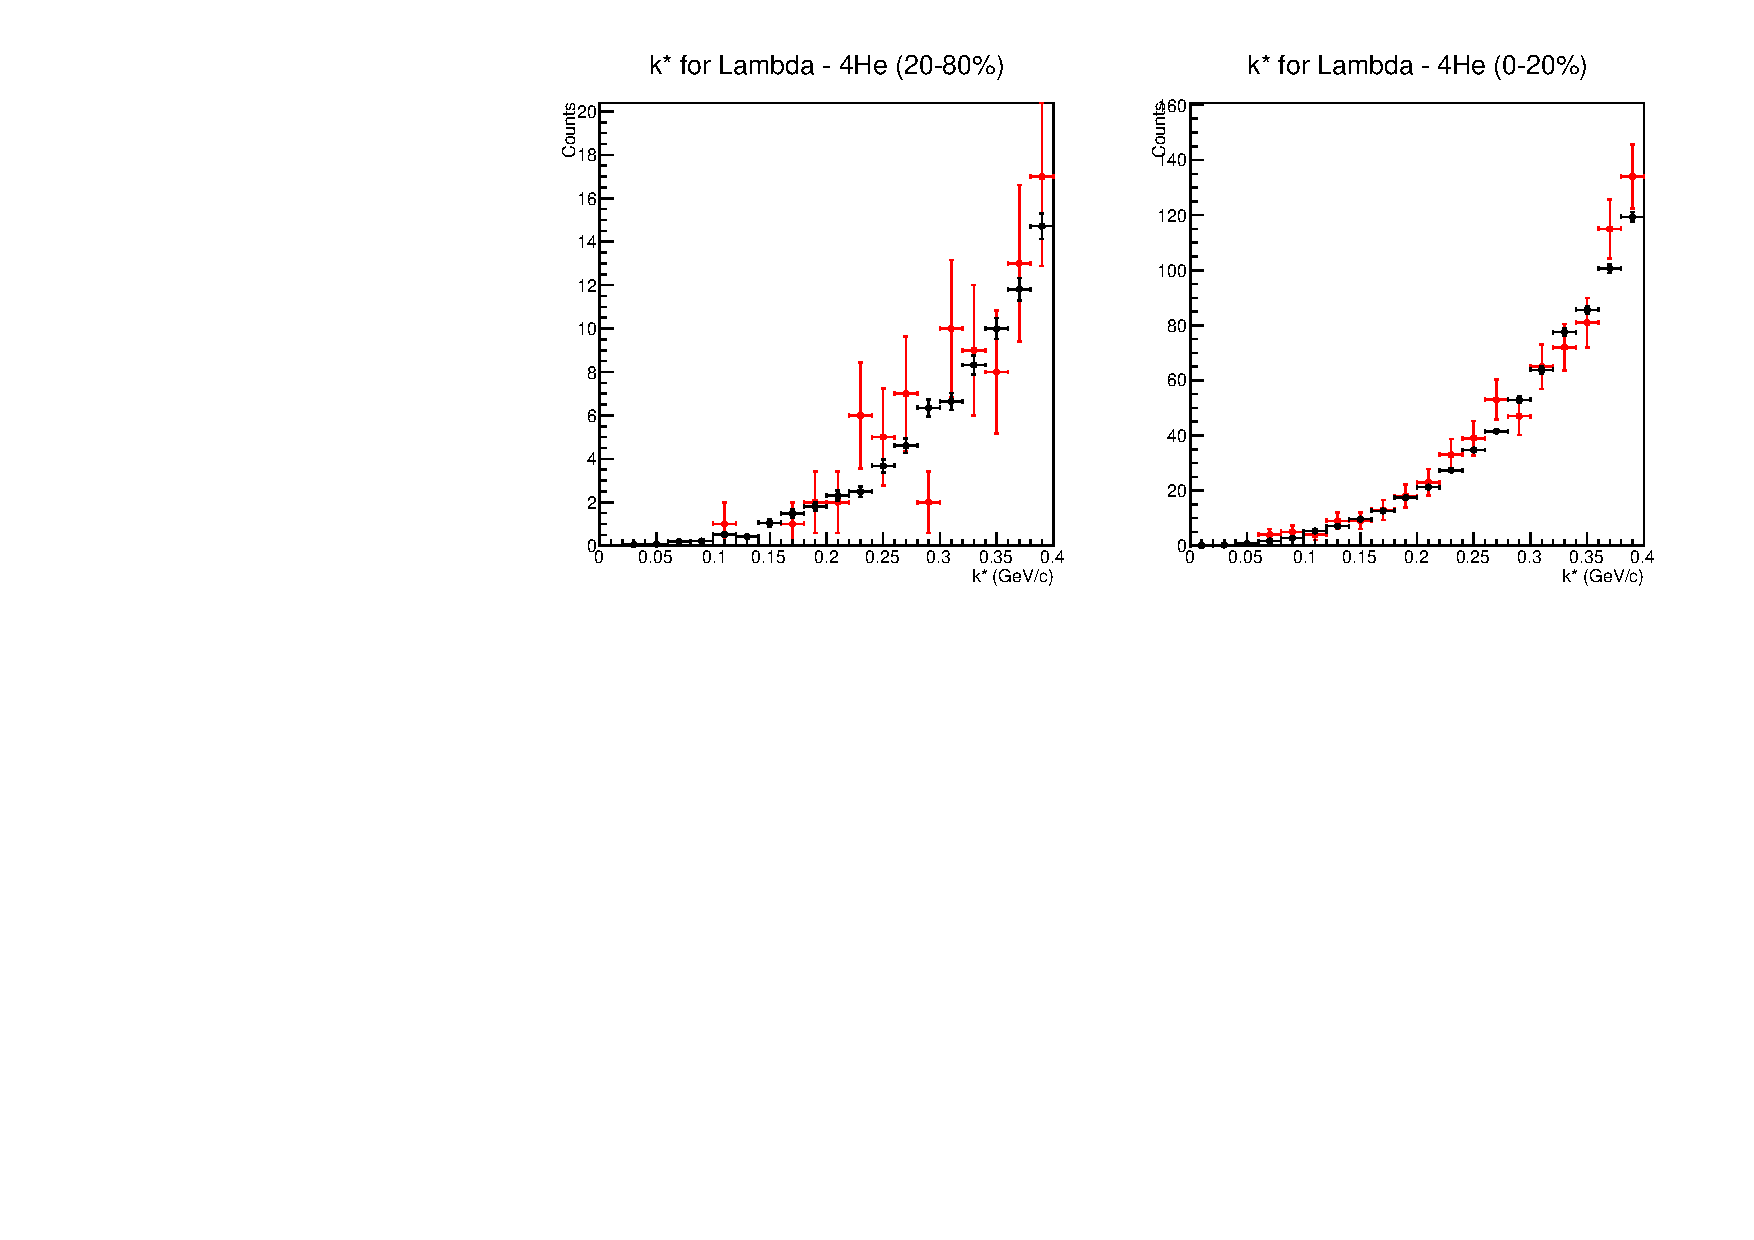
\includegraphics[width=\textwidth,page=1]{kstar_sum_CFsub_4He.pdf}
\caption{SE and ME in the signal mass gate.}
\end{minipage}
\hfill
\begin{minipage}{0.49\textwidth}\centering
\includegraphics[width=\textwidth,page=2]{kstar_sum_CFsub_4He.pdf}
\caption{Uncorrected signal-gate CF.}
\end{minipage}
\end{figure}
\begin{figure}[!ht]\centering
\begin{minipage}{0.49\textwidth}\centering
\includegraphics[width=\textwidth,page=5]{kstar_sum_CFsub_4He.pdf}
\caption{Signal-gate CF and summed-sideband CF.}
\end{minipage}
\hfill
\begin{minipage}{0.49\textwidth}\centering
\includegraphics[width=\textwidth,page=6]{kstar_sum_CFsub_4He.pdf}
\caption{CFsub using the current inclusive-purity proxy.}
\end{minipage}
\end{figure}
\clearpage\section{Method 3: mass-fit signal yields}
\begin{figure}[!ht]\centering
\begin{minipage}{0.49\textwidth}\centering
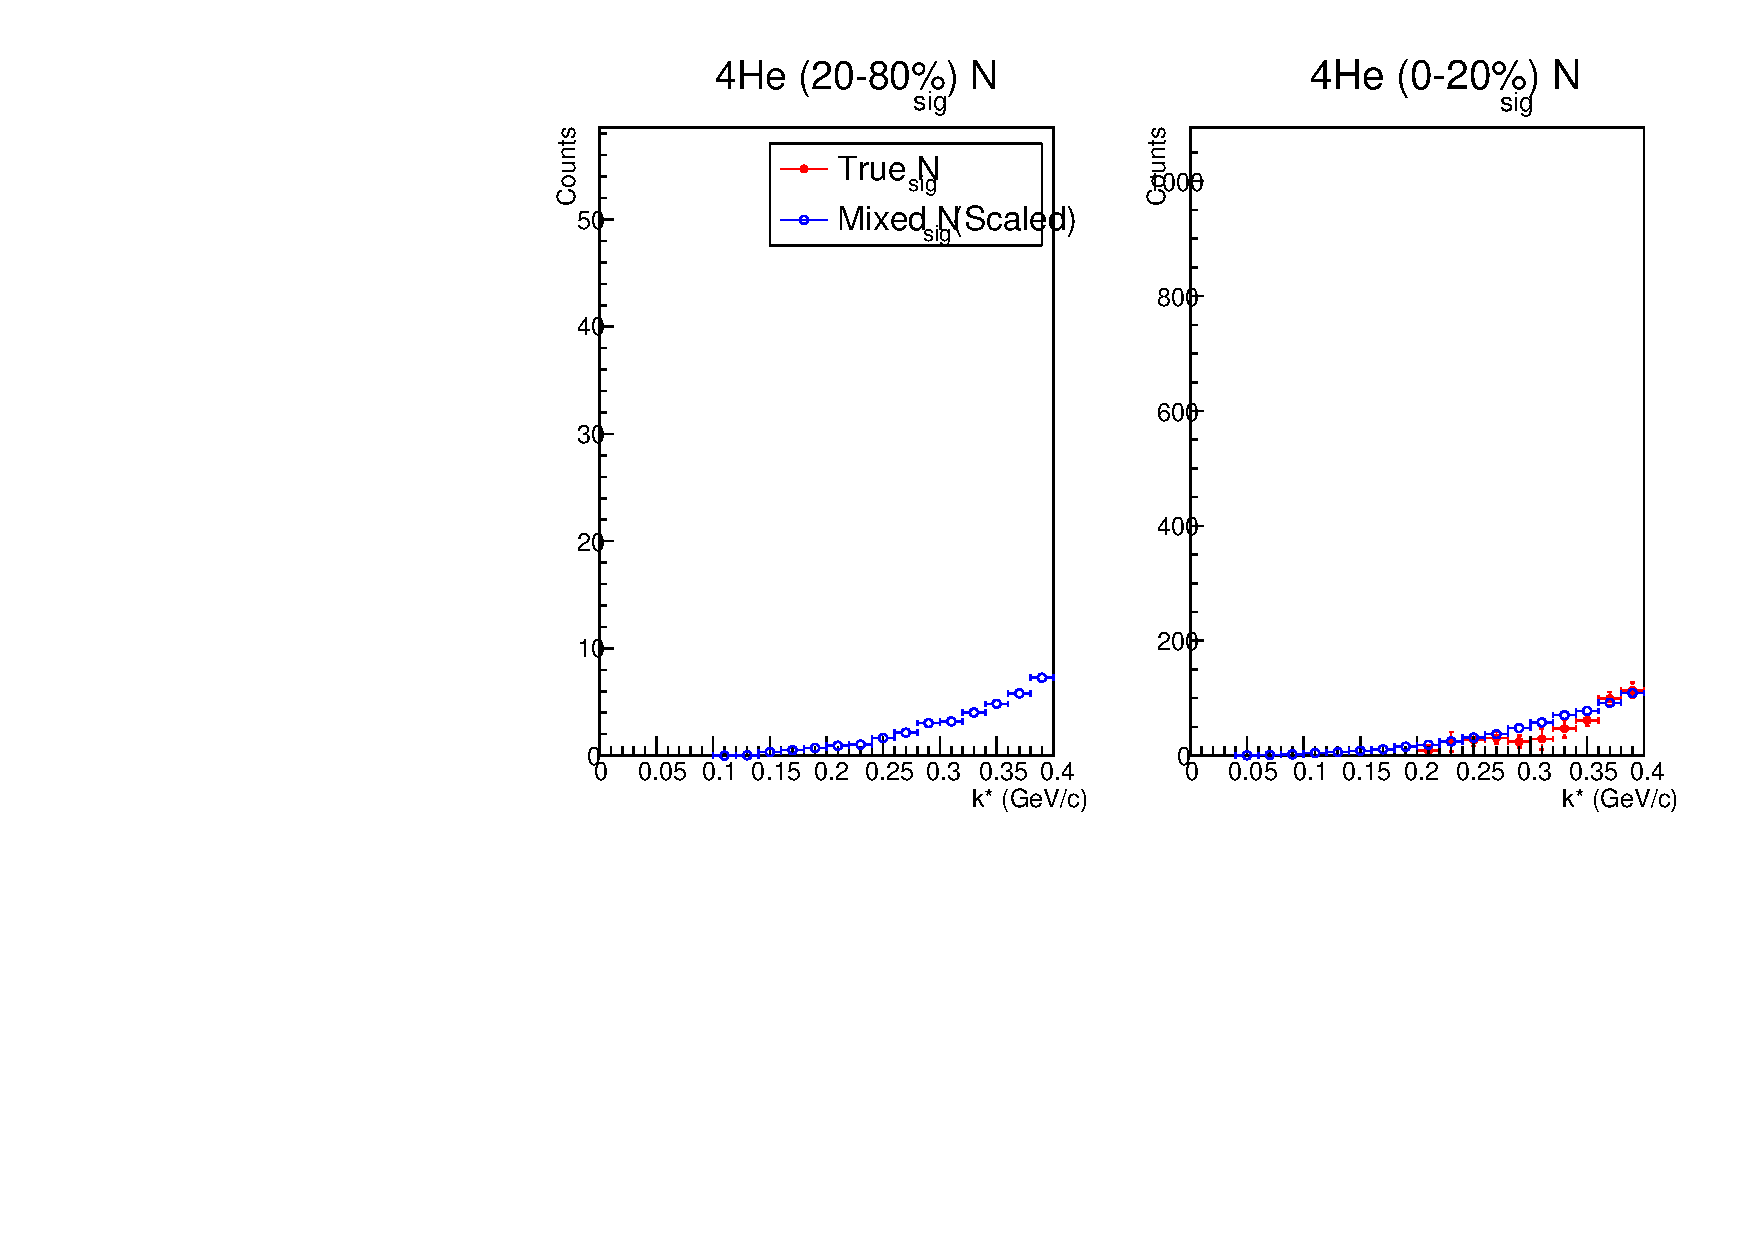
\includegraphics[width=\textwidth,page=1]{kstar_sum_CFsub_method3_4He.pdf}
\caption{Mass-fit SE and ME signal yields.}
\end{minipage}
\hfill
\begin{minipage}{0.49\textwidth}\centering
\includegraphics[width=\textwidth,page=2]{kstar_sum_CFsub_method3_4He.pdf}
\caption{SE and ME fitted purity versus $k^*$.}
\end{minipage}
\end{figure}
\begin{figure}[!ht]\centering
\includegraphics[width=0.85\textwidth,page=3]{kstar_sum_CFsub_method3_4He.pdf}
\caption{Normalized fitted-signal-yield ratio. Fit quality must be checked independently.}
\end{figure}
\clearpage\section{Method 5: sliding-window comparison}
Both fine-centrality figures below show all nine centralities. The 0--5\% bin is the bottom-right panel; page 2 is a purity summary, not a single-centrality page.
\begin{figure}[!ht]\centering
\begin{minipage}{0.49\textwidth}\centering
\includegraphics[width=\textwidth,page=2]{kstar_cent_CFsub_method3_4He.pdf}
\caption{Method 3 purity in nine centrality bins.}
\end{minipage}
\hfill
\begin{minipage}{0.49\textwidth}\centering
\includegraphics[width=\textwidth,page=2]{kstar_cent_CFsub_method5_4He.pdf}
\caption{Method 5 sliding-window purity in the same bins.}
\end{minipage}
\end{figure}
\begin{figure}[!ht]\centering
\begin{minipage}{0.49\textwidth}\centering
\includegraphics[width=\textwidth,page=3]{kstar_sum_CFsub_method3_4He.pdf}
\caption{Method 3 grouped CF.}
\end{minipage}
\hfill
\begin{minipage}{0.49\textwidth}\centering
\includegraphics[width=\textwidth,page=3]{kstar_sum_CFsub_method5_4He.pdf}
\caption{Method 5 grouped CF; adjacent-bin covariance is omitted.}
\end{minipage}
\end{figure}
\clearpage\section{Exploratory Lednicky--Lyuboshits fits}
The blue fits hold $a_0=4.01$ fm and $r_{\rm eff}=1.84$ fm fixed and fit $R$ and a normalization. The red fits also vary $a_0$ and $r_{\rm eff}$. These reproduce the existing model/sign convention, not an independently validated interaction extraction. The fit interval is $0<k^*<0.4$ GeV/$c$: only about 20 bins of width 20 MeV/$c$ are available before invalid-bin exclusions. Four free parameters can therefore be weakly constrained. Parameter bounds, covariance quality and fit status matter in addition to the displayed $\chi^2$/ndf.
\begin{figure}[!ht]\centering
\begin{minipage}{0.49\textwidth}\centering
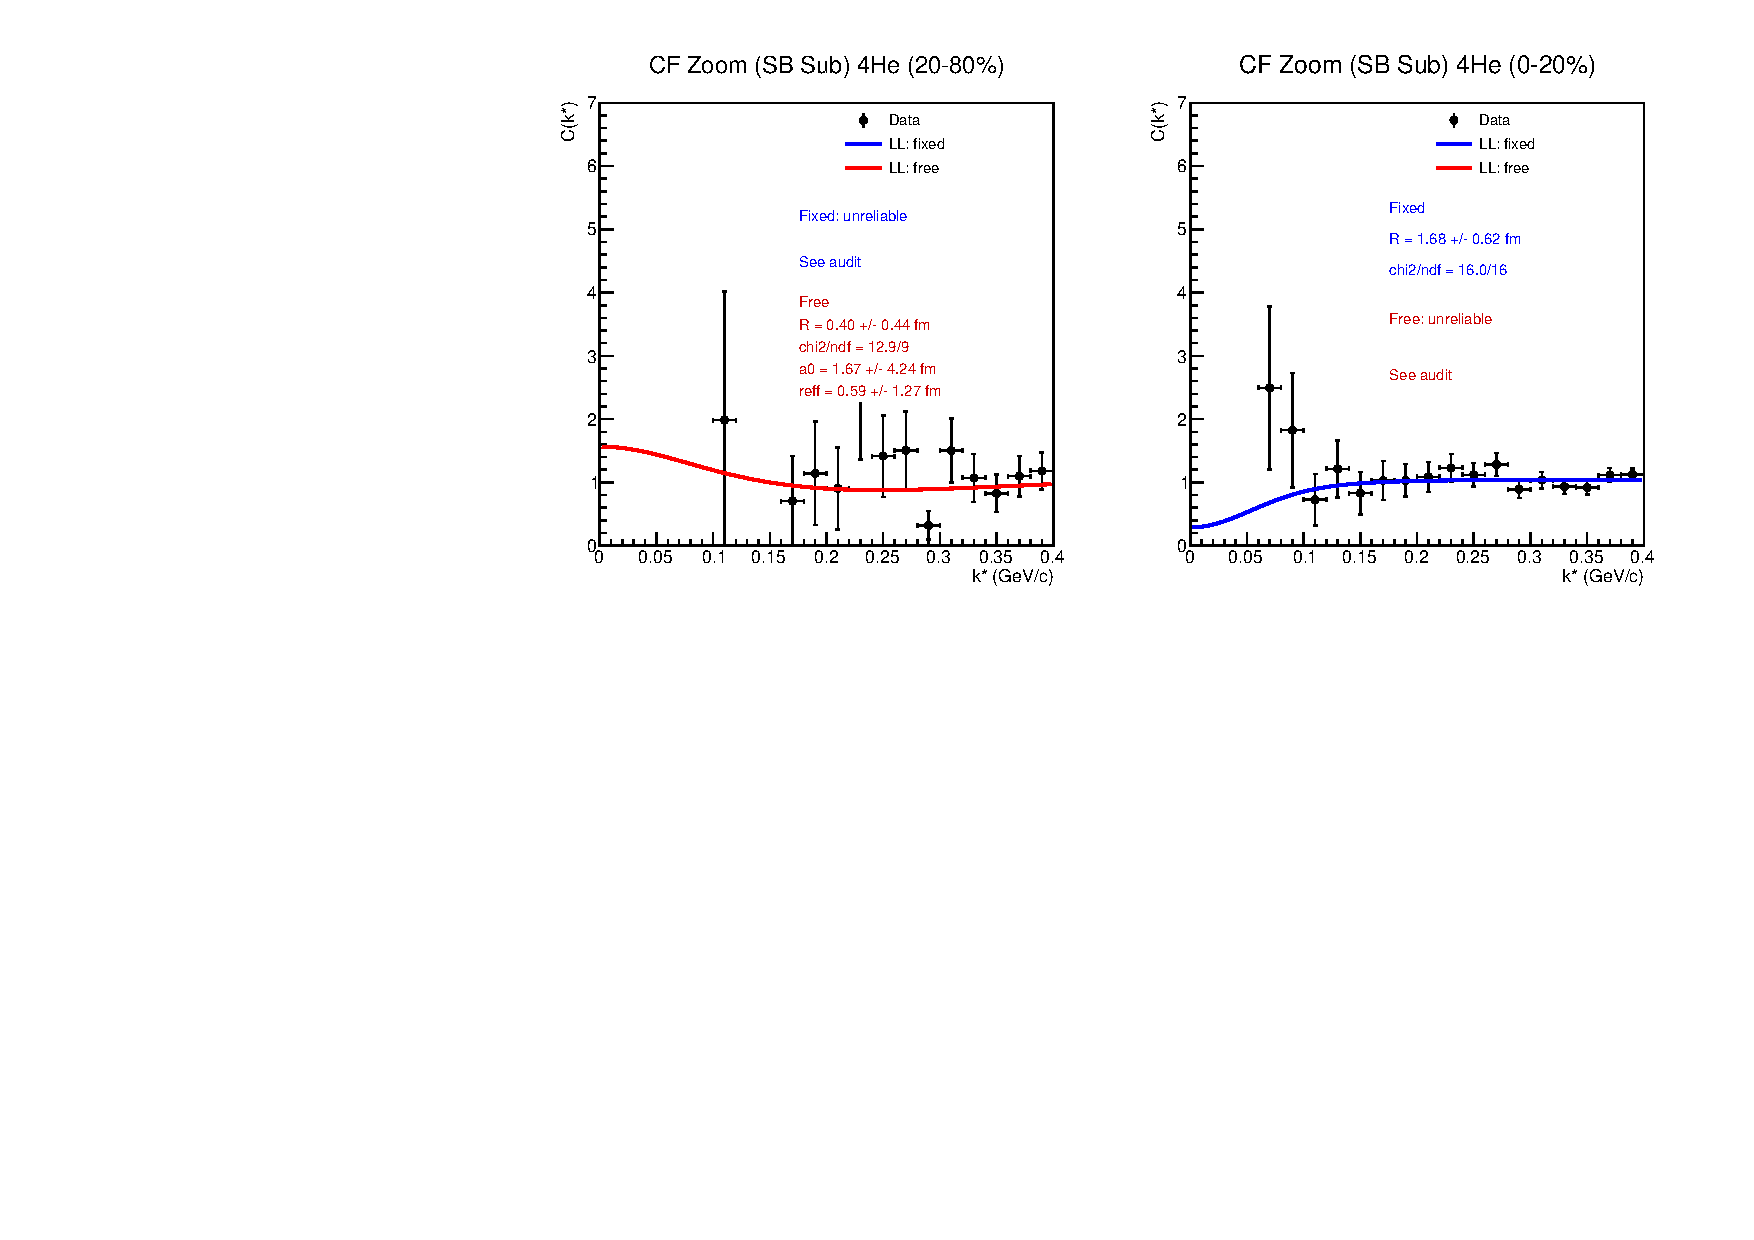
\includegraphics[width=\textwidth,page=1]{Fit_LL_4He.pdf}
\caption{LL fits to raw-SB-subtracted CFs.}
\end{minipage}
\hfill
\begin{minipage}{0.49\textwidth}\centering
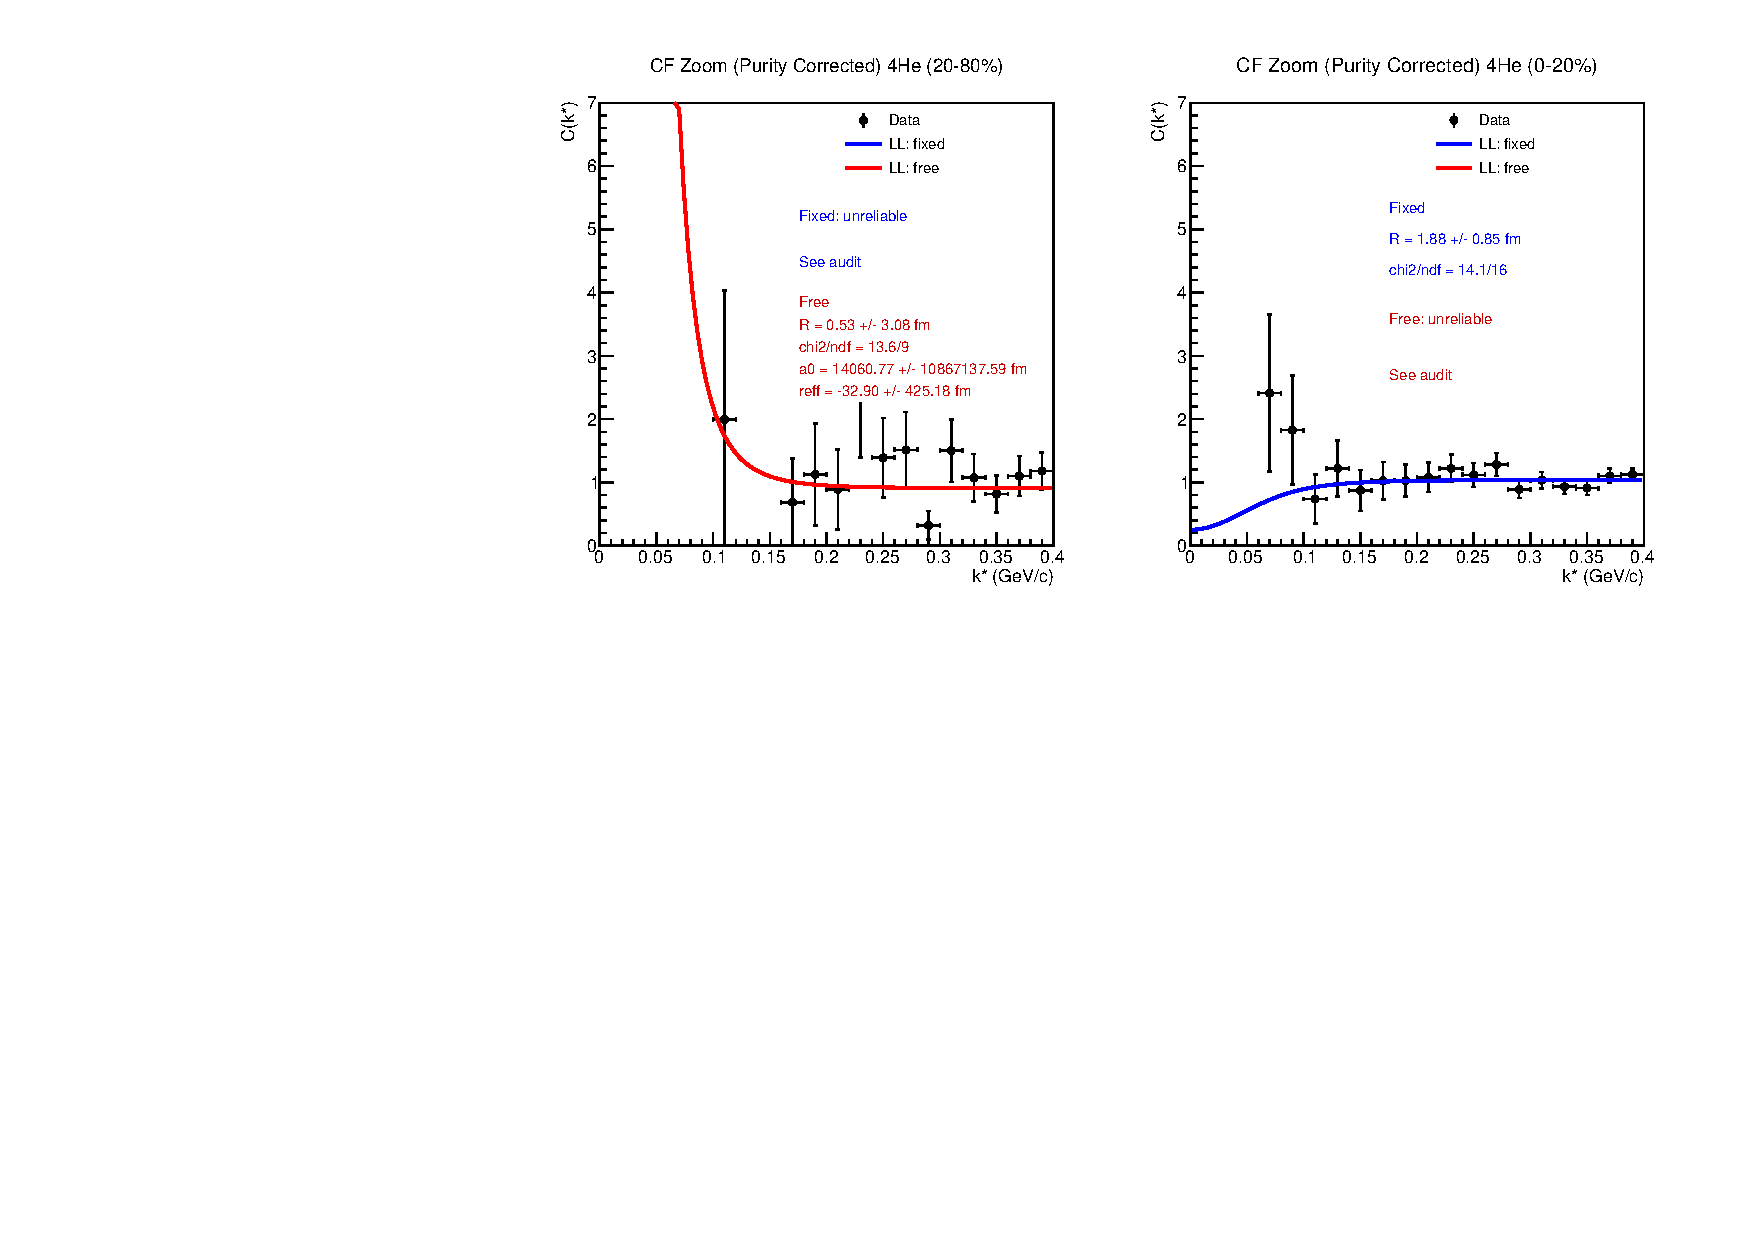
\includegraphics[width=\textwidth,page=1]{Fit_LL_CFsub_4He.pdf}
\caption{LL fits to constant-purity CFsub CFs.}
\end{minipage}
\end{figure}
\begin{figure}[!ht]\centering
\begin{minipage}{0.49\textwidth}\centering
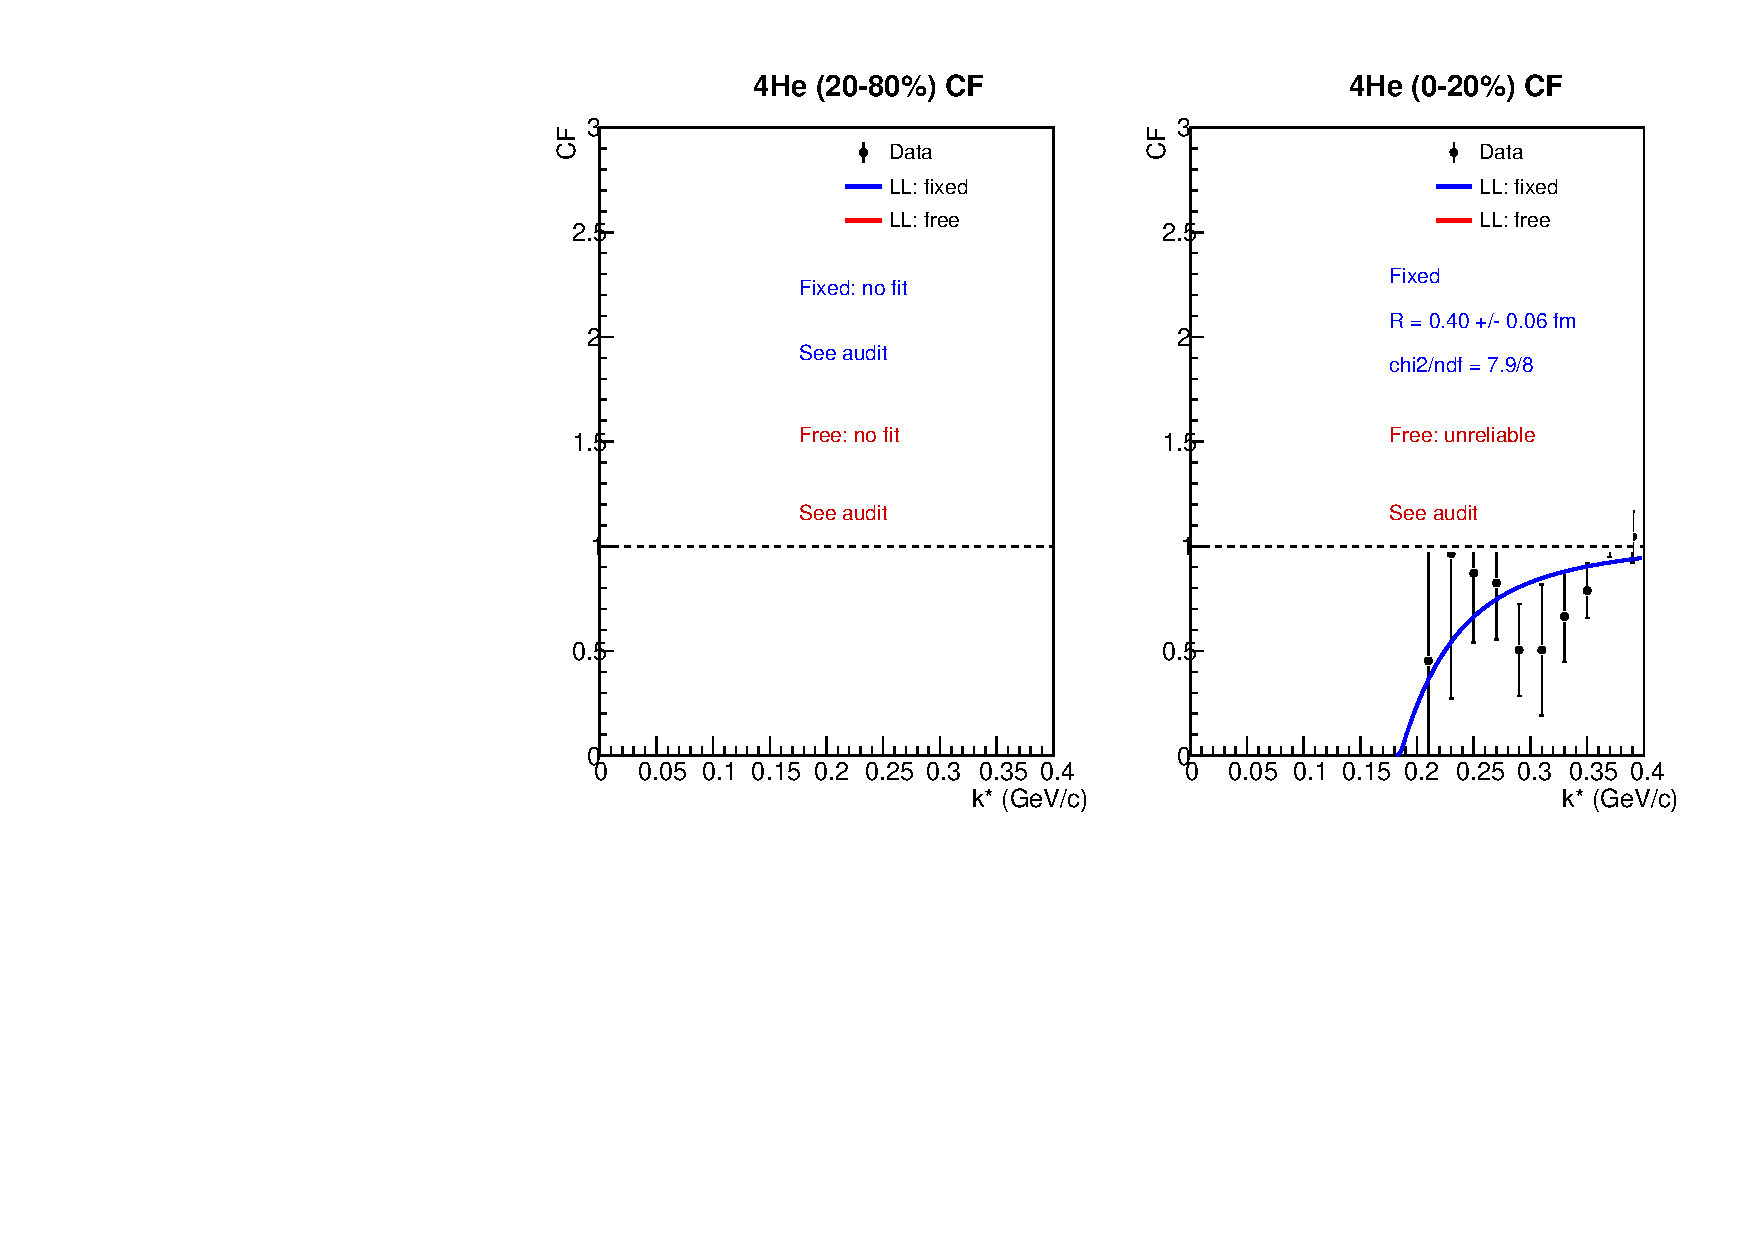
\includegraphics[width=\textwidth,page=1]{Fit_LL_method3_4He.pdf}
\caption{LL fits to Method 3 CFs.}
\end{minipage}
\hfill
\begin{minipage}{0.49\textwidth}\centering
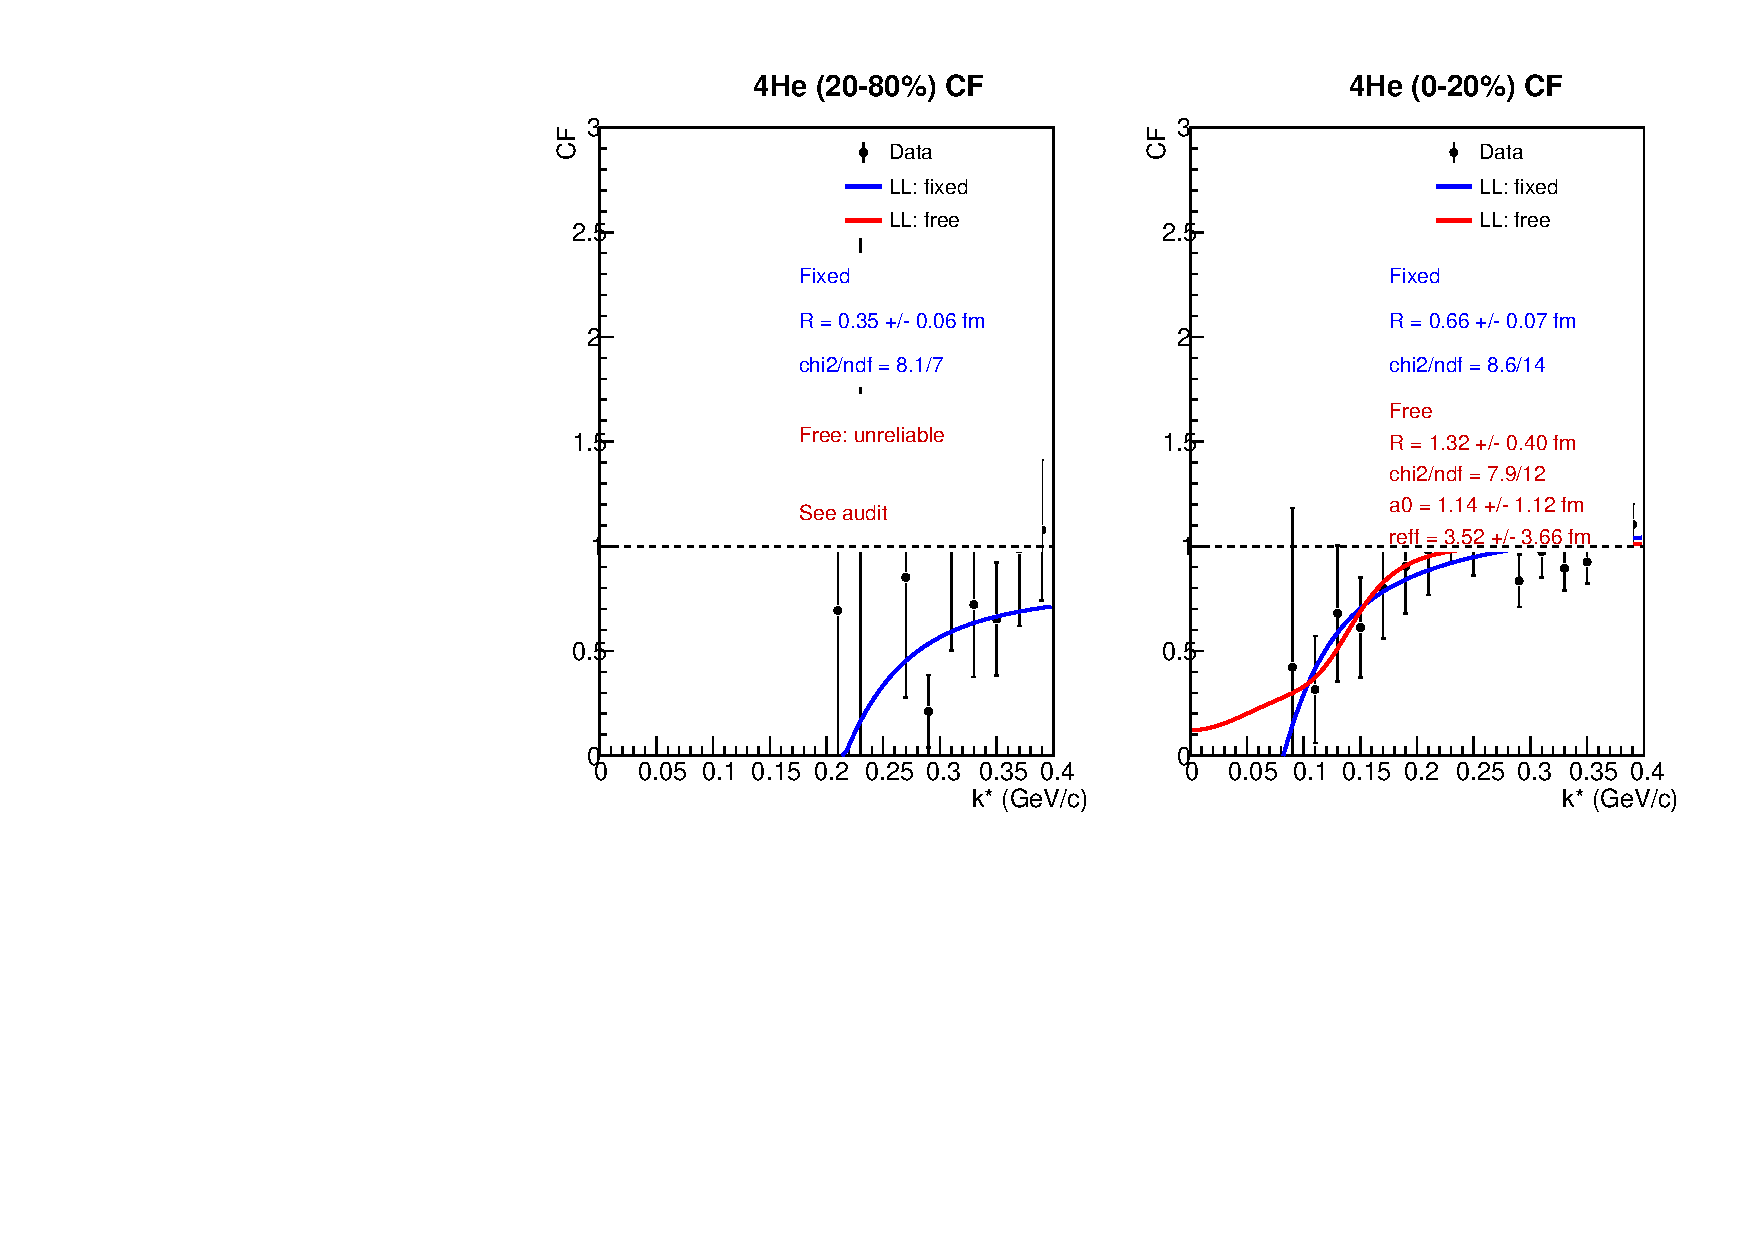
\includegraphics[width=\textwidth,page=1]{Fit_LL_method5_4He.pdf}
\caption{LL fits to Method 5 CFs; window covariance is not fitted.}
\end{minipage}
\end{figure}
\clearpage\section{Additional centrality groups}
The following pages use the same groups for every method: 0--10\%, 10--20\% and 20--60\%. This corrects the inconsistent third-group definitions in some legacy macros.
\begin{figure}[!ht]\centering
\begin{minipage}{0.49\textwidth}\centering
\includegraphics[width=\textwidth,page=12]{kstar_sum_4He.pdf}
\caption{SBsub, second group set.}
\end{minipage}
\hfill
\begin{minipage}{0.49\textwidth}\centering
\includegraphics[width=\textwidth,page=12]{kstar_sum_CFsub_4He.pdf}
\caption{Constant-purity CFsub, second group set.}
\end{minipage}
\end{figure}
\begin{figure}[!ht]\centering
\begin{minipage}{0.49\textwidth}\centering
\includegraphics[width=\textwidth,page=6]{kstar_sum_CFsub_method3_4He.pdf}
\caption{Method 3, second group set.}
\end{minipage}
\hfill
\begin{minipage}{0.49\textwidth}\centering
\includegraphics[width=\textwidth,page=6]{kstar_sum_CFsub_method5_4He.pdf}
\caption{Method 5, second group set.}
\end{minipage}
\end{figure}
\clearpage\section{LL fit audit and reproducibility}
Fit status 0 alone does not establish model adequacy. Covariance status and boundary flags are retained separately below. Repeated optimizer calls are reduced to the last result for each fit object. Full parameters and diagnostics remain in the TSV files.
{\small\begin{longtable}{lrrrr}\hline Mass-fit macro & Total & Accepted & Boundary & Rejected\\\hline\endhead
draw\_sum\_CFsub\_method3 & 500 & 396 & 65 & 104\\
draw\_sum\_CFsub\_method5 & 500 & 451 & 40 & 49\\
draw\_CFsub\_method3 & 900 & 426 & 92 & 474\\
draw\_CFsub\_method5 & 900 & 561 & 77 & 339\\
Fit\_sum\_CFsub\_method3 & 500 & 396 & 65 & 104\\
Fit\_sum\_CFsub\_method5 & 500 & 451 & 40 & 49\\
\hline\end{longtable}}
Accepted here means only the implemented numerical checks passed; it is not a goodness-of-fit or physics validation. Boundary cases are included in accepted counts and are shown separately as warnings.
For object \texttt{fit1\_s\_g}, $a_0$ and $r_{\rm eff}$ are fixed; \texttt{fit2\_s\_g} is the all-free fit. The zero-based group-set index $s=0$ means (20--80\%, 0--20\%) and $s=1$ means (0--10\%, 10--20\%, 20--60\%); $g$ is the position in that list.
{\scriptsize\begin{longtable}{llrrrr}\hline Macro / fit & Object & Status & Cov. & Bound & $R$ (fm)\\\hline\endhead
SBsub & fit1\_0\_0 & 0 & 3 & 1 & 6*\\
SBsub & fit1\_0\_1 & 0 & 3 & 0 & 1.679\\
SBsub & fit1\_1\_0 & 0 & 3 & 0 & 1.577\\
SBsub & fit1\_1\_1 & 0 & 3 & 1 & 6*\\
SBsub & fit1\_1\_2 & 0 & 3 & 1 & 6*\\
SBsub & fit2\_0\_0 & 0 & 3 & 0 & 0.4018\\
SBsub & fit2\_0\_1 & 0 & 3 & 1 & 6*\\
SBsub & fit2\_1\_0 & 0 & 3 & 0 & 5.999\\
SBsub & fit2\_1\_1 & 0 & 3 & 0 & 0.5727\\
SBsub & fit2\_1\_2 & 0 & 3 & 0 & 0.512\\
CFsub & fit1\_0\_0 & 0 & 3 & 1 & 6*\\
CFsub & fit1\_0\_1 & 0 & 3 & 0 & 1.879\\
CFsub & fit1\_1\_0 & 0 & 3 & 0 & 1.71\\
CFsub & fit1\_1\_1 & 0 & 3 & 1 & 6*\\
CFsub & fit1\_1\_2 & 0 & 3 & 1 & 6*\\
CFsub & fit2\_0\_0 & 0 & 3 & 0 & 0.527\\
CFsub & fit2\_0\_1 & 0 & 3 & 1 & 6*\\
CFsub & fit2\_1\_0 & 0 & 3 & 1 & 6*\\
CFsub & fit2\_1\_1 & 0 & 3 & 0 & 0.5757\\
CFsub & fit2\_1\_2 & 0 & 3 & 0 & 0.5294\\
CFsub\_method3 & fit1\_0\_0 & -1 & -1 & 0 & not fitted\\
CFsub\_method3 & fit1\_0\_1 & 0 & 3 & 0 & 0.3987\\
CFsub\_method3 & fit1\_1\_0 & 0 & 3 & 0 & 0.3843\\
CFsub\_method3 & fit1\_1\_1 & 0 & 3 & 0 & 0.289\\
CFsub\_method3 & fit1\_1\_2 & -1 & -1 & 0 & not fitted\\
CFsub\_method3 & fit2\_0\_0 & -1 & -1 & 0 & not fitted\\
CFsub\_method3 & fit2\_0\_1 & 4 & 2 & 1 & 0.1*\\
CFsub\_method3 & fit2\_1\_0 & 0 & 3 & 0 & 0.7155\\
CFsub\_method3 & fit2\_1\_1 & -1 & -1 & 0 & not fitted\\
CFsub\_method3 & fit2\_1\_2 & -1 & -1 & 0 & not fitted\\
CFsub\_method5 & fit1\_0\_0 & 0 & 3 & 0 & 0.3484\\
CFsub\_method5 & fit1\_0\_1 & 0 & 3 & 0 & 0.659\\
CFsub\_method5 & fit1\_1\_0 & 0 & 3 & 0 & 0.5923\\
CFsub\_method5 & fit1\_1\_1 & 0 & 3 & 0 & 0.3467\\
CFsub\_method5 & fit1\_1\_2 & 0 & 3 & 0 & 0.3484\\
CFsub\_method5 & fit2\_0\_0 & 0 & 3 & 1 & 0.1*\\
CFsub\_method5 & fit2\_0\_1 & 0 & 3 & 0 & 1.322\\
CFsub\_method5 & fit2\_1\_0 & 0 & 3 & 0 & 1.206\\
CFsub\_method5 & fit2\_1\_1 & 0 & 3 & 0 & 0.3265\\
CFsub\_method5 & fit2\_1\_2 & 0 & 2 & 0 & 0.1023\\
\hline\end{longtable}}
An asterisk marks an unreliable optimizer result. Not fitted suppresses initial parameters left behind when too few valid points were available. Even unmarked fits remain exploratory and omit the covariance sources noted above.
{\small\textbf{Reproduction records:} Measurements: \path{inspect.json}; macros/settings: \path{macro_manifest.json}; input/configuration: \path{run_state.json}; fit diagnostics: \path{logs/}; figure hashes/pages: \path{report_metadata.json}. Commands and full figure index: \path{README.md}.}
\end{document}
